\section{Example}

\subsection{5 Prism example}

The example model is comprised of five anomalous rectangular prisms embedded in a uniform halfspace. There are three surface prisms simulating near-surface distortions, and two buried prisms simulating deeper targets (see Figure \ref{fig:5prisms}). 

The five blocks from Figure \ref{fig:5prisms} are assigned conductivity and chargeability values in accordance with Table \ref{tabl:properties}.

\begin{table}[ht]
\centering
\begin{tabular}{|c|c|c|}
\hline
ID & Conductivity (mS/m) & Chargeability (\%) \\
\hline
S$_1$ & 10 & 5 \\
\hline
S$_2$ & 5 & 5 \\
\hline
S$_3$ & 0.5 & 5 \\
\hline
B$_1$ & 0.5 & 15 \\
\hline
B$_2$ & 10 & 15 \\
\hline
\end{tabular}
\caption{Electrical conductivity and chargeability, assigned to the 5 blocks contained within the synthetic model.}
\label{tabl:properties}
\end{table}

DC resistivity and IP data are forward modelled for both surface and cross-borehole arrays using the \codeName{DCIPoctreeFwd} code. Three different electrode configurations were were used for both DC and IP data types to show the benfits of a joint inversion using both surface and borehole data. Details of the three survey types are as follows:  

\begin{enumerate}
\item Surface dataset: Pole-dipole arrays with $a=50$m (smallest potential electrode spacing) and $n$ (potential electrode position) ranging from 1 to 6. Eleven east-west lines with a line spacing of 100m were used to cover the core region of the model which is 1km square. In total 1,089 observations were forward modelled using 209 current electrodes.
\item Borehole dataset: Pole-Dipole arrays located within 4 boreholes, whose locations are specified in table \ref{tabl:BHloc}. The data were simulated using a borehole array configuration in which the current electrode is moved down each of the 4 boreholes with 25m steps to the depth of 350m. This results in a total of 51 current electrode locations. For each of the current electrode locations, the potential electrode array, with a 50m spread was placed in each of the remaining three boreholes and moved down to a depth of 350m at 25m intervals resulting in 1,530 forward modelled observations.
\item Combined surface and borehole dataset: A combination of the the above pole-dipole surface and borehole arrays, resulting in 260 current electrodes and 2,619 total forward modelled observations.
\end{enumerate}

\begin{table}[ht]
\centering
\begin{tabular}{|c|c|c|}
\hline
ID & Easting (m) & Northing (m) \\
\hline
A & 200 & 500 \\
\hline
B & 500 & 200 \\
\hline
C & 800 & 500 \\
\hline
D & 500 & 800 \\
\hline
\end{tabular}
\caption{Locations of the synthetic boreholes.}
\label{tabl:BHloc}
\end{table}

Prior to inversion, 5\% white Gaussian noise was added to the forward modelled data, and uncertainties were assigned to be 5\% of the data value plus a small floor. For each of the experiments conducted, most of the inversion parameters were held constant for consistency. Some of these parameters include:
\begin{description}[leftmargin=3.5cm, style=sameline, align=left]
\item[\fileName{octree\_mesh:}] 159,772 cells on an underlaying base mesh which is 128x128x64 cells and has a smallest cell size of 30x30x15 m. 
\item[\fileName{ref. model:}] A uniform halfspace with a conductivity of 0.001 S/m and a chargeability of 0.0001.
\item[\fileName{int. model:}] Same as the reference model.
\item[\fileName{active cells:}] No topography is used and all model cells are active in this example so, the topography and model active cells are both set to \codeName{ALL\_ACTIVE}.  
\item[\fileName{cell weights:}] No cell weights are used (\codeName{NO\_WEIGHTS}). 
\item[\fileName{interface weights:}] No interface weights are used (\codeName{NO\_FACE\_WEIGHTS}). 
\item[\codeName{$\beta$:}] $\beta$ values are set to \codeName{DEFAULT}. 
\item[\codeName{$\alpha$:}] $\alpha$ coefficients ($\alpha_s = 1.0e-5$, $\alpha_x = 1$, $\alpha_y = 1$, $\alpha_z = 1$). This corresponds to a length scale of approximately 316.23 m in all three directions. 
\item[\codeName{chifact:}] 1. 
\item[\codeName{tol\_nl:}] 1.e-2. 
\item[\codeName{mindm:}] 1.e-3.
\item[\codeName{iter\_per\_beta:}] 2. 
\item[\codeName{tol\_ipcg:}] 1.e-2. 
\item[\codeName{max\_iter\_ipcg:}] 15. 
\item[\codeName{$m_{ref}$ change:}] The reference model is not changed at each \codeName{beta\_step} (\codeName{NO\_CHANGE\_MREF}). 
\item[\codeName{smoothing:}] The \codeName{SMOOTH\_MOD\_DIF} option was used in all inversions, so the model objective function is defined by equation(\ref{eq:mof1}) (i.e. the reference model is used in the derivative terms). 
\item[\fileName{bounds:}] For the DC data \codeName{NO\_BOUNDS} were applied, but for the IP data a positivity constraint was enforced using constant bounds (\codeName{BOUNDS\_CONST 0 1}) this forces all recovered chargeability values to be between $[0,1)$.
\end{description}

\subsubsection{DC resistivity inversion of surface data over an octree mesh} 

The first inversion result, which uses only the DC surface data, was carried out using the following input control file. 

\begin{adjustwidth}{-1in}{-1in}
\begin{fileExample}
\begin{tabular}{|ll|}
\hline
octree\_mesh\_11.txt & ! octree mesh file \\
LOC\_XYZ  5prism\_dc.dat & ! data file \\
VALUE  0.001 & ! initial model \\
VALUE  0.001 & ! reference model \\
ALL\_ACTIVE & ! topography active cell file \\
ALL\_ACTIVE & ! model active cell file \\
NO\_WEIGHT & ! cell weighting file\\
NO\_FACE\_WEIGHT & ! interface weighting file\\
DEFAULT & ! \textbar beta\_max; beta\_min; beta\_factor \\
1.0e-5  1.  1.  1. & ! alpha\_s; alpha\_x; alpha\_y; alpha\_z \\
1. & ! chifact \\
1.e-2  1.e-3  2 & ! tol\_nl mindm; iter\_per\_beta \\
1.e-2  15 & ! tol\_ipcg; max\_iter\_ipcg \\
NO\_CHANGE\_MREF & ! change mref \\
SMOOTH\_MOD\_DIF & ! smoothing \\
BOUNDS\_NONE & ! bounds \\
\hline
\end{tabular}
\end{fileExample}
\end{adjustwidth}

\begin{figure}[!ht]
\center
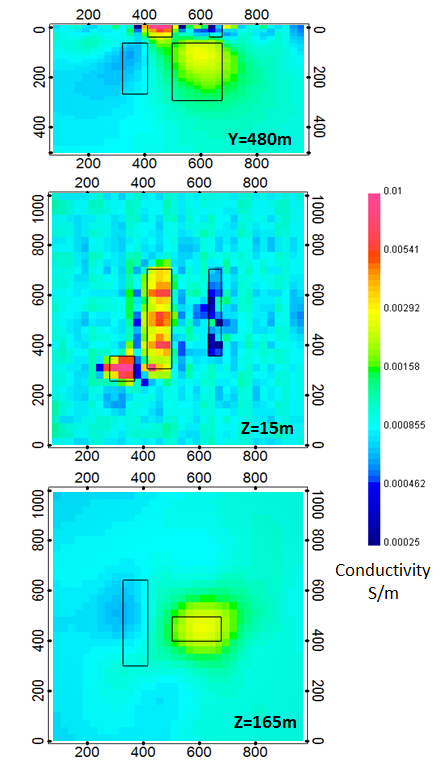
\includegraphics[height=6.25 in]{InvDC}
\caption{The conductivity model recovered from inversion of surface data. Each of the panels shows a different section through the reocovered model. The top panel shows a cross section along Y = 480m, the middle panel is a depth section from a depth of Z = 15m, and the bottom panel shows a second depth section from Z = 165m. The positions of the true prisms are indicated by the black outlines within each model section. While the surface blocks are nicely resolved by the inversion, the deeper blocks only show up as diffuse anomalies whose shape, spatial location, and physical property contrast with the background are not very well defined.}
\label{fig:InvDC}
\end{figure}
  
The inversion converged after 17 beta iterations to a final data misfit of 1.65615E+03. The recovered model is shown in Figure \ref{fig:InvDC}. While the recovered model is quite similar to the true model, especially in the near surface regions its ability to resolve the deeper blocks is clearly limited. Within each of the sections presented the black outlines show the location of the blocks in the true model. 

The top panel of Figure \ref{fig:InvDC} shows a cross section through the recovered model at Y = 480m. In this view, the itersected conductive surface block is well resolved, but the thinner resistive surface block is slightly more difficult to pick out among the near surface artifacts (more refined inversion models could be devised to remove or smooth out many of these near surface anomalies using cell and interface weighting). While the presence of the deeper blocks is clearly visible in the top panel the recovered anomalies are smeared out and lack definition.

The second panel from the top shows a depth slice through the model at a depth of 15m. In this view all 3 of the surface blocks are well fairly well resolved. As should be expected the conductive blocks are slightly better resolved than the resistive block. The boundaries of the resistive surface block are somewhat blurred by the presence near surface artifacts (most of which appear to be more resistive than the background in this particular section). 

The bottom panel of Figure \ref{fig:InvDC} shows another depth slice through the recovered model. This section cross-cuts the 2 deeper blocks at a depth of Z = 165m. As was observed in the top panel, the deeper blocks are clearly visible but somewhat diffuse in that they are spread over a region larger than that of the true block and lack sharp boundaries. In this section the deep conductive block is much better resolved than the deep resistive block. Although the conductive anomaly is slightly larger than the true block it is centered about the true location. In contrast, the deep resistive anomaly is shifted slightly to the west and north of the true block location and is smeared out extensively towards the western edge of the model. As a result of the resistive anomaly's larger size there is less of a physical property contrast between the anomaly and the background. For this type of surface data the observed decrease in model resolution at depth is anticipated, since we have a limited separation between current and potential electrodes. 

\subsubsection{IP inversion of surface data over an octree mesh}

The following IP inversion result was derived using the same surface electrode array as the previous DC inversion to recover a chargeability model of the subsurface. The input control file for this inversion has the following form:

\begin{adjustwidth}{-1in}{-1in}
\begin{fileExample}
\begin{tabular}{|ll|}
\hline
octree\_mesh\_11.txt & ! octree mesh file\\
LOC\_XYZ  5prism\_ip.dat & ! data file \\
VALUE  0.001 & ! initial model \\
VALUE  0.001 & ! reference model \\
inv.con & ! refernce conductivity model \\
ALL\_ACTIVE & ! topography active cell file \\
ALL\_ACTIVE & ! model active cell file \\
NO\_WEIGHT & ! cell weighting file\\
NO\_FACE\_WEIGHT & ! interface weighting file\\
DEFAULT & ! \textbar beta\_max; beta\_min; beta\_factor \\
1.0e-5  1.  1.  1. & ! alpha\_s; alpha\_x; alpha\_y; alpha\_z \\
1. & ! chifact \\
1.e-2  1.e-3  2  & ! tol\_nl; mindm; iter\_per\_beta \\
1.e-2  15 & ! tol\_ipcg; max\_iter\_ipcg \\
NO\_CHANGE\_MREF & ! change mref \\
SMOOTH\_MOD\_DIF  & ! smoothing \\
BOUNDS\_CONST  0  1 & ! bounds \\
\hline
\end{tabular}
\end{fileExample}
\end{adjustwidth}

\begin{figure}[!ht]
\center
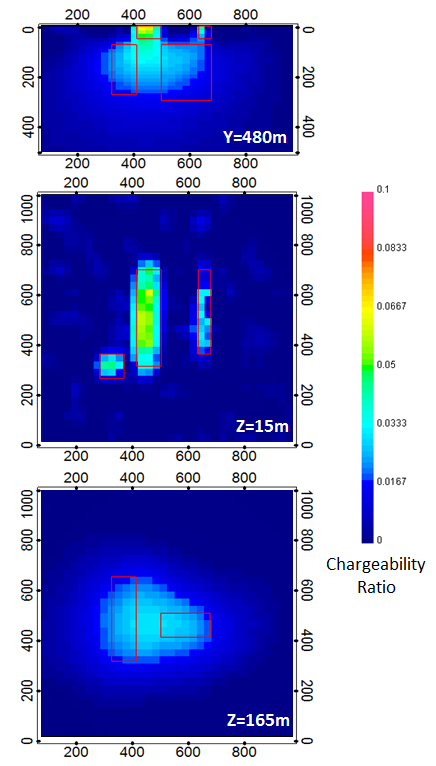
\includegraphics[height=6.25 in]{InvIP}
\caption{The chargeability model recovered from inversion of surface data shown using 3 different section views which transect the 5 chargeable blocks in the true model. The top panel shows a cross section along Y = 480m, while the middle panel shows a depth section at of Z = 15m, and the bottom panel shows a second depth section from Z = 165m. The positions of the true blocks are indicated by the red outlines within each model section. While the surface blocks are nicely resolved by the inversion, the deeper blocks only show up as a single diffuse anomaly. In addition to the lateral smearing of the chargeable blocks at depth, vertical smearing has also connected the shallow chargeable blocks with those at depth indicating that the resolution of the model decays rapidly with depth.}
\label{fig:InvIP}
\end{figure}

Primary differences between this inversion and the previous surface data inversion that was preformed using DC data are restircted to the reference model and bound constraints. For the IP surface data inversion  a uniform halfspace with a chargeability of 0.0001 (near-zero) is used for the reference model and the sensitivity calculation was done using the recovered conductivity model from the DC surface data inversion (see Figure \ref{fig:InvDC}). While no bound ocnstraints were applied in the DC surface data inversion, a positivity constraint is applied for all of the IP inversions presented here. Constant bounds were set in the input file (\codeName{BOUNDS\_CONST 0 1}, setting the lower bound to zero and upper bound to 1) to prevent the recovered chargeability values from being negative.

The IP surface data inversion converged after 6 beta iterations to a a final data misfit of 1.30090E+03. The recovered model is shown in Figure \ref{fig:InvIP}. While the recovered  model offers a good representation of the large scale chargeability distribution, many of the details are lost. Within each of the sections presented the red outlines show the location of the blocks in the true model. 

The top panel of Figure \ref{fig:InvIP} shows a cross section through the recovered model at Y = 480m. In this view, the wider of the 2 itersected surface blocks is well resolved, while the thinner chargeable surface block is slightly more difficult to resolve. Although the presence of the deeper blocks is clearly visible in the top panel the recovered anomalies are smeared together into a single anomaly at depth which appears to connect with the chargeable surface anomalies. Despite the fact that the deeper blocks are more chargeable than the surface blocks, the inversion result indicates the opposite as a result of the larger near surface sensitivities.

The middle panel shows a depth slice through the model at a depth of 15m. In this view all 3 of the surface blocks are well resolved. The response from the eastern most chargeable surface block is fainter than the other surface blocks because it is thinner. When compared with the DC inversion of surface data (see Figure \ref{fig:InvDC}) the near surface artifacts in the IP inversion are lower in amplitude, making it easier to resolve all three surface blocks. 

The bottom panel of Figure \ref{fig:InvIP} shows another depth slice through the recovered model which cuts the 2 deeper blocks at a depth of Z = 165m. As was observed in the top panel, the deeper blocks are have been smeared together to form a single diffuse anomaly. From this inversion result it is impossible to tell that the true model contained 2 separate chargeable blocks at depth. As this result clearly illustrates the surface data alone is not capable of accurately resolving the chargeable bodies at depth. 


\subsubsection{DC inversion of borehole data over an octree mesh}

Since the DC inversion based on surface data (see Figure \ref{fig:InvDC}) did not resolve the anomalous blocks at depth very precisely, here we preform another inversion using data from 4 separate boreholes. The input control file for this inversion has the following form:  

\begin{adjustwidth}{-1in}{-1in}
\begin{fileExample}
\begin{tabular}{|ll|}
\hline
octree\_mesh\_11.txt & ! octree mesh file \\
LOC\_XYZ  5prism\_dc\_borehole.dat & ! data file \\
VALUE  0.001 & ! initial model \\
VALUE  0.001 & ! reference model \\
ALL\_ACTIVE & ! topography active cell file \\
ALL\_ACTIVE & ! model active cell file \\
NO\_WEIGHT & ! cell weighting file\\
NO\_FACE\_WEIGHT & ! interface weighting file\\
DEFAULT & ! \textbar beta\_max; beta\_min; beta\_factor \\
1.0e-5  1.  1.  1. & ! alpha\_s; alpha\_x; alpha\_y; alpha\_z \\
1. & ! chifact \\
1.e-2  1.e-3  2 & ! tol\_nl; mindm; iter\_per\_beta \\
1.e-2  15 & ! tol\_ipcg; max\_iter\_ipcg \\
NO\_CHANGE\_MREF & ! change mref \\
SMOOTH\_MOD\_DIF & ! smoothing \\
BOUNDS\_NONE & ! bounds \\
\hline
\end{tabular}
\end{fileExample}
\end{adjustwidth}

\begin{figure}[!ht]
\center
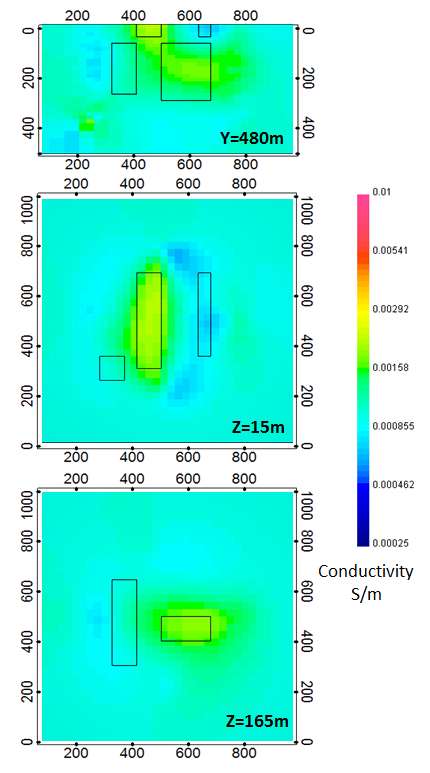
\includegraphics[height=6.25 in]{InvDC_BH}
\caption{The electrical conductivity model recovered from the inversion of DC borehole data. The position of the true blocks are indicated by the black outlines. When compared with the inversion result using the DC surface data (Figure \ref{fig:InvDC}) there is a general decrease in model resolution as a result of decreased sensitivites in region surrounding the blocks due to the borehole survey geometry. While the most significant decreases in the model resoultion are seen in the near surface, this inversion result also does a very poor job of resolving the deep resistive block.}
\label{fig:InvDC_BH}
\end{figure}

This inversion converged after 15 beta iterations to a a final data misfit of 1.49948E+03. The recovered model is shown in Figure \ref{fig:InvDC_BH}. Within each of the sections presented the black outlines show the location of the blocks within the true model. When compared with the inversion of DC surface data in Figure (\ref{fig:InvDC}) there is a significant decrease in resolution throughout the model and the amplitude of the recovered anomalies significantly under estimates the conductivity contrast between the blocks and the background. 

The top panel of Figure \ref{fig:InvDC_BH} shows a cross section through the recovered model at Y = 480m. Here, both of the surface blocks are visible but they lack sharp boundaries and the large conductive surface block has been smeared downwards to connect with the conductive block at depth. While there is a resistive anomaly in the vacinity of the deep resistive block, the recovered anomaly is shifted to the west.

The second panel from the top shows a depth slice through the model at a depth of 15m. In this section only the large surface conductive block is resolved. The small western most conductive surface block is not recovered at all, and the thin resistive surface block to the east has been highly distorted to form a chevron like shape which points to the east. While the large surface conductive block is the best resolved surface block it has still bled slighly into the background region surrounding the block and lacks sharp boundaries. 

The bottom panel of Figure \ref{fig:InvDC_BH} shows another depth slice through the recovered model. This section cross-cuts the 2 deeper blocks at a depth of Z = 165m. At this depth the deep conductive block is recovered, but only a faint trace of resistive material is present to the west of the true location of the deep resistive block. Although the conductive anomaly is slightly larger than the true block it is centered about the true location. As in the above panels the recovered anomalies have very diffuse boundaries.


\subsubsection{IP inversion of borehole data over an octree mesh}

Using the same survey geometry as in DC borehole data inversion above (Figure \ref{fig:InvDC_BH}) an IP inversion was also done to see how well we could resolve the 5 chargeable blocks. Below is the input control file that was used for this IP inversion.

\begin{adjustwidth}{-1in}{-1in}
\begin{fileExample}
\begin{tabular}{|ll|}
\hline
octree\_mesh\_11.txt & ! octree mesh file \\
LOC\_XYZ  5prism\_ip\_borehole.dat & ! data file \\
VALUE  0.001 & ! initial model \\
VALUE  0.001 & ! reference model \\
inv.con & ! refernce conductivity model \\
ALL\_ACTIVE & ! topography active cell file \\
ALL\_ACTIVE & ! model active cell file \\
NO\_WEIGHT & ! cell weighting file\\
NO\_FACE\_WEIGHT & ! interface weighting file\\
DEFAULT & ! \textbar beta\_max; beta\_min; beta\_factor \\
1.0e-5  1.  1.  1. & ! alpha\_s; alpha\_x; alpha\_y; alpha\_z \\
1. & ! chifact \\
1.e-2  1.e-3  2 & ! tol\_nl; mindm; iter\_per\_beta \\
1.e-2  15 & ! tol\_ipcg; max\_iter\_ipcg \\
NO\_CHANGE\_MREF & ! change mref \\
SMOOTH\_MOD\_DIF & ! smoothing \\
BOUNDS\_CONST  0  1 & ! bounds \\
\hline
\end{tabular}
\end{fileExample}
\end{adjustwidth}

\begin{figure}[!ht]
\center
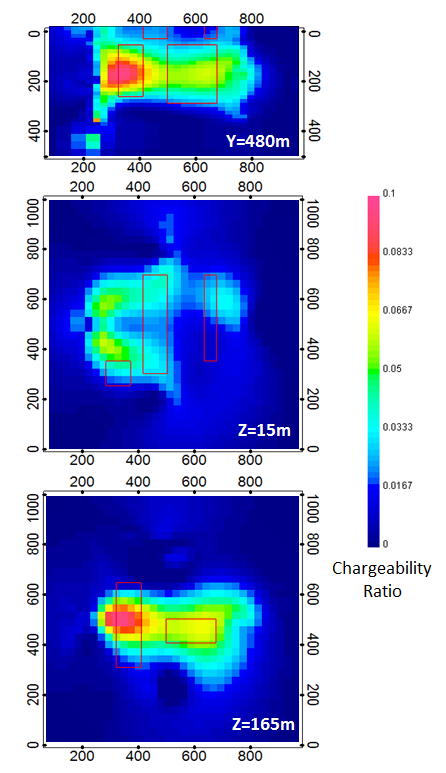
\includegraphics[height=6.25 in]{InvIP_BH}
\caption{The chargeability model recovered from inversion of surface data shown using 3 different section views which transect the 5 chargeable blocks in the true model. The top panel shows a cross section along Y = 480m, while the middle panel shows a depth section at of Z = 15m, and the bottom panel shows a second depth section from Z = 165m. The positions of the true prisms are indicated by the red outlines within each model section. The conductivity from the DC borehole data inversion (see Figure \ref{fig:InvDC_BH}) was used to calculate sensitivities. The depth resolution of this model has significantly increased compared to surface data inversion (Figure \ref{fig:InvIP}), however this was done at the expense of the near surface resolution.}
\label{fig:InvIP_BH}
\end{figure}

As in the previous IP inversion, the sensitivity was calculated using the conductivity model recovered from the corresponing DC inversion (i.e. DC borehole inversion, see Figure \ref{fig:InvDC_BH}) and upper and lower bounds were set to 0 and 1 respectively to enforce a positivity constraint on the recovered chargeability.

This inversion converged after 27 beta iterations to a a final data misfit of 1.52016E+03. The recovered model is shown in Figure \ref{fig:InvIP_BH}. Within each of the sections presented the red outlines show the location of the blocks in the true model. Although the recovered model does a fair job of resolving the deep chargeable blocks it is unable to recover any of the surface blocks. 

The top panel of Figure \ref{fig:InvIP_BH} shows a cross section through the recovered model at Y = 480m. In this view, a high chargeability anomaly is centred at depth around the 2 deep blocks, but extensive smearing is visible in both lateral and vertical directions. The region of highest chargeability is centred about the eastern deep chargeable block. This anomaly has been smeared laterally to the east so that it connects with the other deep chargeable block and vertically up to the surface. It does not appear as though any of the surface blocks have been recovered. 

The middle panel shows a depth slice through the model at a depth of 15m. This section shows to inability of this inversion result to resolve any of the surface blocks. Based on the location and shape of the high chargeability anomaly visible in this section it appears as though this anomaly is an artifact of the inversion produced by the vertical smearing of the deep chargeable blocks up to the surface. As one would expect with the borehole data the near surface sensitivites are very small when contrasted with the surface data IP inversion (see Figure \ref{fig:InvIP}).


The bottom panel of Figure \ref{fig:InvIP_BH} shows another depth slice through the recovered model which cuts the 2 deeper blocks at a depth of Z = 165m. As was observed in the top panel, the deeper blocks are have been smeared together to form a single diffuse anomaly with a region of higher chargeability centred around the western block. From this inversion result it is very difficult to tell that the true model contained 2 separate chargeable blocks at depth. The fact that the deep western chargeable block in the recovered model has a higher charageability than the eastern block must be a result of the north-south orientation of the western block and its proxity to the boreholes since both deep blocks have the same chargeability.


\subsubsection{DC resistivity inversion of joint surface and borehole data sets over an octree mesh} 

Since neither the surface or borehole DC data were able to adequately resolve all 5 blocks, a joint inverion was done using both data sets. The input control file for this inversion has the following form:
 
\begin{adjustwidth}{-1in}{-1in}
\begin{fileExample}
\begin{tabular}{|ll|}
\hline
octree\_mesh\_11.txt & ! octree mesh file \\
LOC\_XYZ  5prism\_dc\_joint.dat & ! data file \\
VALUE  0.001 & ! initial model \\
VALUE  0.001 & ! reference model \\
ALL\_ACTIVE & ! topography active cell file \\
ALL\_ACTIVE & ! model active cell file \\
NO\_WEIGHT & ! cell weighting file\\
NO\_FACE\_WEIGHT & ! interface weighting file\\
DEFAULT & ! \textbar beta\_max; beta\_min; beta\_factor \\
1.0e-5  1.  1.  1. & ! alpha\_s; alpha\_x; alpha\_y; alpha\_z \\
1. & ! chifact \\
1.e-2  1.e-3  2 & ! tol\_nl; mindm; iter\_per\_beta \\
1.e-2  15 & ! tol\_ipcg; max\_iter\_ipcg \\
NO\_CHANGE\_MREF & ! change mref \\
SMOOTH\_MOD\_DIF & ! smoothing \\
BOUNDS\_NONE & ! bounds \\
\hline
\end{tabular}
\end{fileExample}
\end{adjustwidth}

\begin{figure}[!ht]
\center
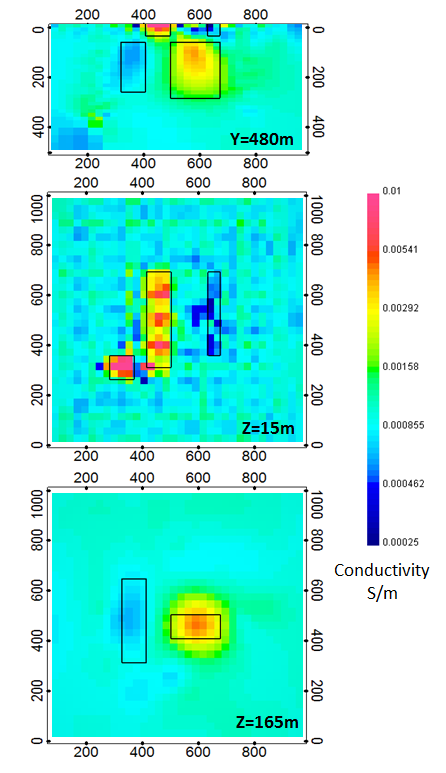
\includegraphics[height=6.25 in]{InvDC_JN}
\caption{As anticipated the recovered model from the joint inversion of surface and borehole DC data does the best job of resolving the location of all 5 of the blocks in the true synthetic model. The position of the true blocks are indicated by the black outlines. When compared with the inversion result of the DC surface data (see Figure \ref{fig:InvDC}) there is a significant increase in model resolution at depth due to the incorporation of the borehole data. The near surface model resolution does not appear to have changed significantly as a result of the joint inversion.}
\label{fig:InvDC_JN}
\end{figure}

The inversion converged after 23 beta iterations to a final data misfit of 2.45176E+03. The recovered model is shown in Figure \ref{fig:InvDC_JN}. Within each of the sections presented the black outlines show the location of the blocks in the true model. While there is not a substantial improvement in the near surface model resolution when compared to the DC surface data inversion (see Figure \ref{fig:InvDC}), the deeper conductive and resistive blocks are much better resolved. 

The top panel of Figure \ref{fig:InvDC_JN} shows a cross section through the recovered model at Y = 480m. In this view, the itersected conductive surface block is very well resolved, but the thinner resistive surface block is slightly obscured by near surface artifacts (more refined inversion models could be devised to remove or smooth out many of these near surface anomalies using cell and interface weighting). Although the general size and location of the deeper blocks in well constrained they still lack sharp boundaries.

The second panel from the top shows a depth slice through the model at Z = 15m. In this view all 3 of the surface blocks are well fairly well resolved. As should be expected the conductive blocks are slightly better resolved than the resistive block. The boundaries of the resistive surface block are somewhat difficult to discern as a result of near surface artifacts, most of which appear to be more resistive than the background. 

The bottom panel of Figure \ref{fig:InvDC_JN} shows another depth slice through the recovered model which cuts through the 2 deeper blocks at a depth of Z = 165m. While the recovered anomalies lack sharp outlines and have been slightly smeared to create circular and oval shaped anomalies. This joint DC inversion result does a far better job of resolving the deep blocks than either the DC surface or DC borehole data inversions (see Figures \ref{fig:InvDC} and \ref{fig:InvDC_BH}). The deep resistive block is still shifted slightly to the west in the recovered model, but its north-south location is better defined and the extent of the smearing is dramatically reduced.


\subsubsection{IP inversion of joint surface and borehole data sets over an octree mesh} 

To see if a joint inversion of the surface and borehole IP data would help to better resolve the chargeable blocks in the true model this final inversion was run using the following input control file:

\begin{adjustwidth}{-1in}{-1in} 
\begin{fileExample}
\begin{tabular}{|ll|}
\hline
octree\_mesh\_11.txt & ! octree mesh file \\
LOC\_XYZ  5prism\_ip\_joint.dat & ! data file \\
VALUE  0.001 & ! initial model \\
VALUE  0.001 & ! reference model \\
inv.con & ! refernce conductivity model \\
ALL\_ACTIVE & ! topography active cell file \\
ALL\_ACTIVE & ! model active cell file \\
NO\_WEIGHT & ! cell weighting file\\
NO\_FACE\_WEIGHT & ! interface weighting file\\
DEFAULT & ! \textbar beta\_max; beta\_min; beta\_factor \\
1.0e-5  1.  1.  1. & ! alpha\_s; alpha\_x; alpha\_y; alpha\_z \\
1. & ! chifact \\
1.e-2  1.e-3  2 & ! tol\_nl; mindm; iter\_per\_beta \\
1.e-2  15 & ! tol\_ipcg; max\_iter\_ipcg \\
NO\_CHANGE\_MREF & ! change mref \\
SMOOTH\_MOD\_DIF & ! smoothing \\
BOUNDS\_CONST  0  1 & ! bounds \\
\hline
\end{tabular}
\end{fileExample}
\end{adjustwidth}

\begin{figure}[!ht]
\center
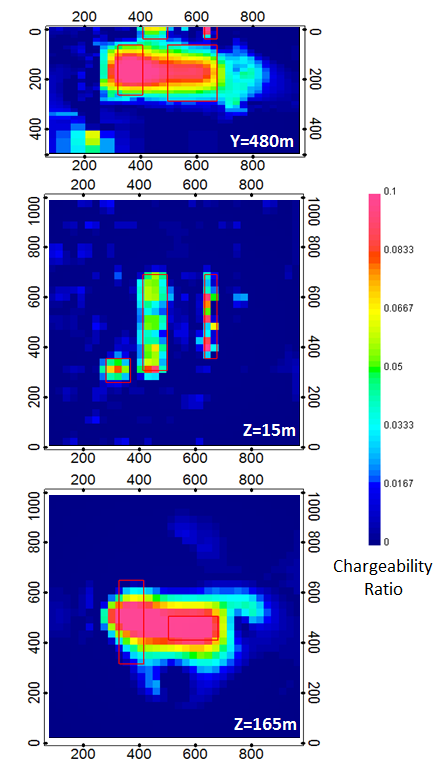
\includegraphics[height=6.25 in]{InvIP_JN}
\caption{The chargeability model recovered from the joint inversion of surface and borehole IP data is shown using 3 different section views which transect the 5 chargeable blocks in the true model. The top panel shows a cross section along Y = 480m, while the middle panel shows a depth section at of Z = 15m, and the bottom panel shows a second depth section from Z = 165m. The positions of the true prisms are indicated by the red outlines within each model section. The conductivity from the joint DC data inversion (see Figure \ref{fig:InvDC_JN}) was used to calculate sensitivities. Significant improvements in the model resolution (both in the near surface and at depth) are apparent when you compare the joint IP data inversion result to that of the surface or borehole IP data inversions.}
\label{fig:InvIP_JN}
\end{figure}

As in the previous IP inversions, the sensitivity was calculated using the conductivity model recovered from the corresponing DC inversion (i.e. DC joint inversion, see Figure \ref{fig:InvDC_JN}) and upper and lower bounds were set to 0 and 1 respectively to enforce a positivity constraint on the recovered chargeability.

This IP inversion converged after 27 beta iterations to a a final data misfit of 2.56821E+03. The recovered model is shown in Figure \ref{fig:InvIP_JN}. Within each of the sections presented the red outlines show the location of the blocks in the true model. The recovered  model offers a good representation of the overall chargeability distribution, and does the best job of resolving the 5 chargeable blocks contained within the true synthetic model. Despite the significant improvements in model resolution at depth, the recovered model from the joint IP inversion is still incapable of distinguishing the two deep blocks. 

The top panel of Figure \ref{fig:InvIP_JN} shows a cross section through the recovered model at Y = 480m. Here, both of the surface blocks are reasonably well resolved. While the vertical extent of the deeper blocks is clearly defined the recovered anomalies are smeared together into a single anomaly at depth. While some vertical smearing is also present between the large surface block and the conductive anomaly at depth the vertical smearing is not nearly as pervasive as it was in the surface or borehole IP inversions (see Figures \ref{fig:InvIP} and \ref{fig:InvIP_BH}). In this inversionresult it is also possible to descern that the deeper blocks are more chargeable than the surface blocks, while the surface IP inversion indicated the opposite.

The middle panel shows a depth slice through the model at a depth of Z = 15m. In this view all 3 of the surface blocks are well resolved. The response from the eastern most chargeable surface block is smaller than the other surface blocks because it is thinner. When compared with the DC inversion of surface data (see Figure \ref{fig:InvDC}) the near surface artifacts in the IP inversion are lower in amplitude, making it easier to resolve all three surface blocks. Surface interface weighting could be easily applied to remove some of the near surface anomalies and potentially sharpen the recovered surface block boundaries.

The bottom panel of Figure \ref{fig:InvIP_JN} shows another depth slice through the recovered model. This section cross-cuts the 2 deeper blocks at a depth of Z = 165m. As was observed in the top panel, the deeper blocks are have been smeared together to form a single anomaly whose vertical extent is fairly well defined. Although the joint surface and borehole IP data inversion was still unable to resolve the 2 chargeable blocks at depth, it still produces the chargeabilty model which is the most similar to the true model.  


